        \clearpage
        \begin{figure*}[ht]
            \pdfbookmark[2]{ID 01}{figure_id_01}
        	\centering
            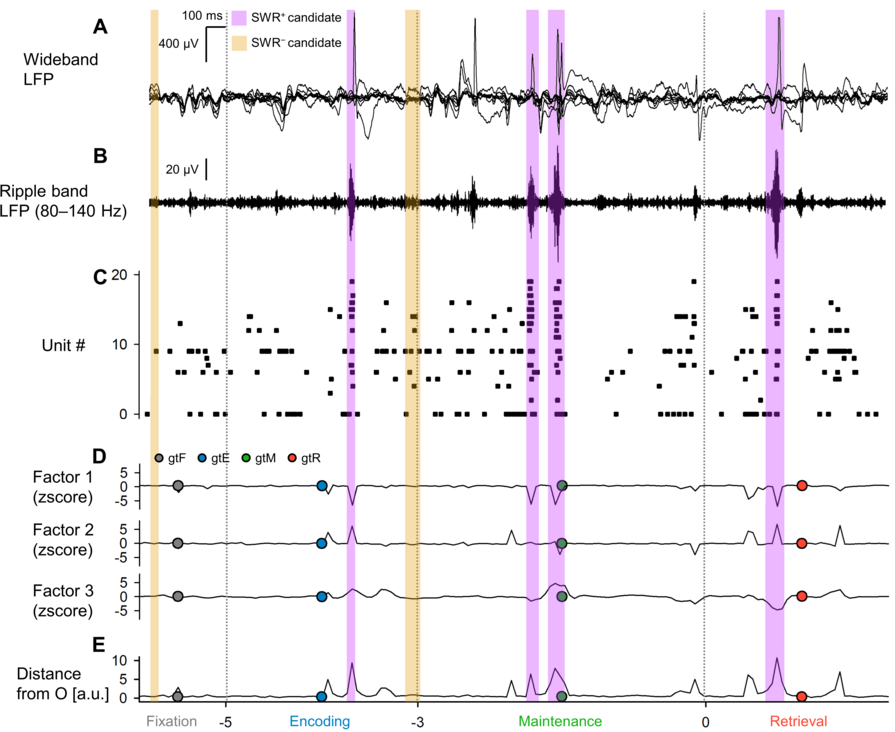
\includegraphics[width=1\textwidth]{./src/figures/.png/Figure_ID_01.png}
        	\caption{\textbf{
Local field potential (LFP), multiunit activity, and neural trajectory of the hippocampus during a modified Sternberg task
}
\smallskip
\\
\textbf{\textit{A.}} Representative wideband LFP traces iEEG signals recorded in the left hippocampal head. The subject conducted a modified Sternberg working memory task, including fixation (1 s, \textit{gray}), encoding (2 s, \textit{blue}), maintenance (3 s, \textit{green}), and retrieval (2 s, \textit{red}). \textbf{\textit{B.}} The corresponding ripple band LFP traces. \textbf{\textit{C.}} The raster plot of multiunit spikes estimated from the LFP traces using a spike sorting algorithm \cite{niediek_reliable_2016}. \textbf{\textit{D.}} Neural trajectory calculated by GPFA on spike counts per unit with 50-ms bins. The dot circles show the coordinate of geometric median for each phase. \textbf{\textit{E.}} Trajectory distance from the origin $O$. Note that \textit{purple} and \textit{yellow} rectangles shows the timings for SWR$^+$ candidates and SWR$^-$ candidates (control for SWR$^+$), respectively.
}
% width=1\textwidth
        	\label{fig:01}
        \end{figure*}
